\documentclass[11pt, a4paper]{article}

% ── Packages ──────────────────────────────────────────────
\usepackage[utf8]{inputenc}
\usepackage[T1]{fontenc}
\usepackage{amsmath, amssymb, amsfonts}
\usepackage{graphicx}
\usepackage[margin=1in]{geometry}
\usepackage{hyperref}
\usepackage[numbers, sort&compress]{natbib}
\usepackage{booktabs}
\usepackage{siunitx}
\usepackage{caption}
\usepackage{float}
\usepackage{xcolor}
\graphicspath{{../figures/}}

% ── Metadata ──────────────────────────────────────────────
\title{\textbf{Selective Qubit Rotation Gate Design in Dispersive cQED:\\
Waveform Optimization, Multi-Branch Limits, and Open-System Performance}}
\author{cQED Autonomous Research Platform \\ Shyam Shankar Quantum Circuits Group}
\date{\today}

\begin{document}

\maketitle

% ══════════════════════════════════════════════════════════
% 1. ABSTRACT
% ══════════════════════════════════════════════════════════
\begin{abstract}
We present a unified study of selective qubit rotation (SQR) gate design in dispersive circuit QED, consolidating three complementary investigations: closed-system waveform optimization with phase compilation, simultaneous multi-branch SQR limits, and open-system performance under realistic noise including multilevel relaxation, Purcell effects, and concurrent readout backaction. The system is a dispersive transmon--storage cavity with $\omega_q/2\pi=\SI{6.150}{GHz}$, $\omega_c/2\pi=\SI{5.241}{GHz}$, $\chi/2\pi=\SI{-2.84}{MHz}$, $\alpha/2\pi=\SI{-255}{MHz}$, and higher-order corrections $\chi'/2\pi=\SI{-21}{kHz}$, $K/2\pi=\SI{-28}{kHz}$.

The main results are: (1)~The conditional-phase SQR target (cphase-SQR) is dramatically easier than the true SQR target, making it the natural baseline primitive. (2)~The cosine-squared envelope achieves the best closed-system performance in the practical regime ($|\chi|T/2\pi\sim 2$--$3$), reaching conditional-phase fidelity $0.999997$ at $|\chi|T/2\pi=3$. (3)~Simultaneous multi-branch SQR with a common Gaussian multitone waveform is \emph{not viable}: the target-branch rotation angle response is $\sim 10^{-4}$, and three independent correction strategies fail to rescue the hard regime. (4)~A cavity-only phase compilation layer provides systematic improvement for single-target SQR on enlarged logical windows ($\Delta F\approx 0.02$) but does not close the gap to branch-local-$Z$ relaxed fidelity, and it fails entirely for structured all-branch short-gate cases. (5)~Under realistic multilevel noise ($T_{1,ge}=\SI{30}{\micro s}$, $T_{1,ef}=\SI{10}{\micro s}$, $n_\mathrm{th,s}=0.02$), the square-family SQR becomes the best parametric baseline with peak realistic-noise target fidelity $0.944$ near $|\chi|T/2\pi=1$. (6)~GRAPE retains a clear noisy-fidelity advantage over parametric baselines ($F=0.978$ at $|\chi|T/2\pi=1$), and (7)~concurrent readout degrades the reduced logical fidelity from $0.822$ to $0.632$ as readout amplitude increases from $0.5$ to $\SI{2.5}{MHz}$.
\end{abstract}

% ══════════════════════════════════════════════════════════
% 2. INTRODUCTION
% ══════════════════════════════════════════════════════════
\section{Introduction}

Selective qubit rotation (SQR) is a foundational primitive for bosonic quantum information processing in dispersive circuit QED~\cite{blais2021circuit,koch2007transmon}. By applying a frequency-selective qubit drive at the Fock-number-shifted qubit frequency $\omega_q + n\chi$, SQR enables Fock-conditioned qubit rotations essential for encoding, decoding, and error-correcting bosonic quantum states~\cite{heeres2015snap,krastanov2015universal}. The dispersive control tradeoff is between selectivity (which improves with longer pulses) and decoherence (which degrades with longer pulses), creating a practical operating window that depends sensitively on the waveform family, the target fidelity metric, and the noise environment.

This unified study addresses three questions that prior work left open. First, which waveform family is optimal in the closed system, and can post-hoc cavity-phase compilation improve strict logical fidelity? Second, is simultaneous multi-branch SQR viable with a common multitone waveform, or is it a fundamentally different control problem? Third, how does the closed-system ranking change under realistic multilevel noise, Purcell effects, storage thermal occupation, and concurrent readout? The answers come from three component investigations consolidated into a single analysis.

\paragraph{Experiment-facing question.}
The practical question is: \emph{which selective primitive should a bosonic cQED experiment actually calibrate and schedule?} We therefore treat SQR not only as a controllability problem, but as an implementation decision problem: which family is the cleanest closed-system benchmark, which family is the best noisy default once ancilla decay matters, which apparent shortcuts are not worth calibration time, and how aggressively SQR can be interleaved with readout before the control primitive stops being useful.

The remainder of the paper is organized as follows. Section~2 defines the shared system model and pulse families. Section~3 presents the closed-system waveform comparison and phase-compilation analysis. Section~4 reports the simultaneous multi-branch study (a negative result). Section~5 covers the open-system replay including noise budgets, Purcell analysis, GRAPE comparison, and three-mode concurrent readout. Section~6 presents validation, and the paper concludes with recommendations and limitations.

% ══════════════════════════════════════════════════════════
% 3. SYSTEM & METHODS
% ══════════════════════════════════════════════════════════
\section{System and Methods}

\subsection{Hamiltonian}

The two-mode dispersive transmon--storage Hamiltonian is
\begin{equation}
\frac{H_0}{\hbar} = \omega_c a^\dagger a + \omega_q b^\dagger b + \frac{\alpha}{2}b^{\dagger 2}b^2 + \chi\,a^\dagger a\,b^\dagger b + \frac{\chi'}{2}(a^\dagger a)^2\,b^\dagger b + \frac{K}{2}(a^\dagger a)^2,
\label{eq:hamiltonian}
\end{equation}
where $a$ is the storage cavity operator, $b$ is the transmon operator, $\alpha$ is the anharmonicity, $\chi$ is the leading dispersive shift, $\chi'$ is the second-order dispersive correction, and $K$ is the cavity self-Kerr.

The three-mode model extends this with a readout resonator:
\begin{equation}
H_\mathrm{3mode} = H_0 + \omega_r c^\dagger c + \chi_r\,c^\dagger c\,b^\dagger b + \chi_{sr}\,a^\dagger a\,c^\dagger c + \kappa_r\,\text{(dissipation)},
\end{equation}
where $c$ is the readout mode operator, $\omega_r/2\pi = \SI{8.597}{GHz}$, $\kappa_r/2\pi = \SI{2.4}{MHz}$, $\chi_r = \chi$, and the baseline uses $\chi_{sr}=0$.

\subsection{Simulation Parameters}

\begin{table}[H]
\centering
\caption{Nominal device parameters shared across all SQR studies.}
\begin{tabular}{@{} l S[table-format=+3.3] l @{}}
\toprule
Parameter & {Value} & Unit \\
\midrule
Qubit frequency $\omega_q/2\pi$ & 6.150 & GHz \\
Storage cavity frequency $\omega_c/2\pi$ & 5.241 & GHz \\
Anharmonicity $\alpha/2\pi$ & -255 & MHz \\
Dispersive shift $\chi/2\pi$ & -2.84 & MHz \\
Second-order shift $\chi'/2\pi$ & -21 & kHz \\
Cavity self-Kerr $K/2\pi$ & -28 & kHz \\
Readout frequency $\omega_r/2\pi$ & 8.597 & GHz \\
Readout linewidth $\kappa_r/2\pi$ & 2.4 & MHz \\
\bottomrule
\end{tabular}
\label{tab:device_params}
\end{table}

\begin{table}[H]
\centering
\caption{Noise and truncation parameters for the open-system study.}
\begin{tabular}{@{} l l l @{}}
\toprule
Parameter & Value & Unit \\
\midrule
Transmon $T_{1,ge}$ & 20--50 & $\mu$s \\
Transmon $T_{1,fe}$ & 5--15 & $\mu$s \\
Storage loss rate $\kappa_s/2\pi$ & 10 & kHz \\
Storage thermal occupation $n_\mathrm{th,s}$ & 0.00--0.10 & --- \\
Transmon truncation $n_\mathrm{tr}$ & 2 (closed) / 3 (open) & levels \\
Cavity truncation $n_\mathrm{cav}$ & 6--10 & Fock states \\
Logical window & $n = 0, \ldots, 3$ & --- \\
\bottomrule
\end{tabular}
\label{tab:noise_params}
\end{table}

\subsection{Target Types and Metrics}

Two SQR target types are compared:
\begin{itemize}
\item \textbf{True SQR}: the strict logical unitary that applies $R_X(\theta)$ on branch $n_0$ and identity on all other branches, with exact phases.
\item \textbf{Conditional-phase SQR (cphase-SQR)}: relaxes the target to allow an independent virtual-$Z$ correction on each Fock branch. This is the physically natural target because the residual Fock-dependent phase can be absorbed into a subsequent SNAP or virtual-$Z$ layer.
\end{itemize}

The primary metric is the strict logical fidelity $F_\mathrm{strict} = |\mathrm{Tr}(U_\mathrm{tgt}^\dagger U_\mathrm{log})|^2/d^2$, with the block-phase-relaxed fidelity $F_\mathrm{block}$ and target-state fidelity used as supplementary diagnostics.

\subsection{Pulse Families}

Four parametric envelope families and GRAPE are compared:
\begin{enumerate}
\item \textbf{Single-tone Gaussian}: area-normalized truncated Gaussian envelope.
\item \textbf{Square}: constant-amplitude selective pulse.
\item \textbf{Cosine-squared (Hann)}: smooth envelope $\propto \cos^2(\pi t/T)$.
\item \textbf{One-segment multitone Gaussian}: common Gaussian envelope with per-branch frequency components.
\end{enumerate}
GRAPE uses piecewise-constant qubit quadratures solved via \texttt{GrapeSolver}~\cite{khaneja2005optimal}.

The corrected-parameterization multitone uses per-tone corrections $(d_\lambda, d_\alpha, \delta\omega)$ with 12~free parameters for 4~branches, optimized by differential evolution followed by adaptive Nelder--Mead.

% ══════════════════════════════════════════════════════════
% 4. RESULTS: CLOSED-SYSTEM WAVEFORM OPTIMIZATION
% ══════════════════════════════════════════════════════════
\section{Closed-System Waveform Optimization and Phase Compilation}

\subsection{Baseline Envelope Hierarchy}

The conditional-phase SQR target is dramatically easier than true SQR. Gaussian conditional-phase fidelity rises from $0.555$ at $|\chi|T/2\pi=0.5$ to $0.998$ at $2.0$ and $0.99999$ at $3.0$. The cosine-squared envelope performs best at intermediate durations, reaching $0.9963$ at $|\chi|T/2\pi=1.5$, $0.9981$ at $2.0$, and $0.999997$ at $3.0$. Leakage stays below $7.4\times 10^{-5}$ across the full scan.

GRAPE confirms that the system is controllable to near-unit fidelity for both targets at all scanned durations ($F_\mathrm{GRAPE}\approx 1$ for cphase-SQR; $>0.987$ for true SQR at $|\chi|T/2\pi\ge 3$).

In the open-system model, the practical optimum shifts to shorter pulses. The cosine-squared pulse peaks at $F=0.9845$ around $|\chi|T/2\pi=1.5$, while Gaussian and multitone peak near $|\chi|T/2\pi=2.0$ at $F\approx 0.9814$.

\subsection{Phase-Compilation Analysis}

\paragraph{Single-target SQR on enlarged windows.}
On an $N=8$ logical window, the extracted cavity-only phase profile is nearly perfectly linear: worst linear-fit RMS error is $4.59\times 10^{-5}$~rad. At $|\chi|T/2\pi=3$, both families give $\phi(n)\approx -0.0684\,n$~rad.

Applying a linear cavity-only phase layer provides systematic improvement:
\begin{itemize}
\item Gaussian: $0.927\to 0.949$ at $|\chi|T/2\pi=3$ ($\Delta F = 0.022$).
\item Cosine-squared: $0.931\to 0.954$ at $|\chi|T/2\pi=3$ ($\Delta F = 0.023$).
\end{itemize}
However, this does not close the full gap to the branch-local-$Z$-relaxed upper bound ($F=0.999998$ for cosine-squared at $|\chi|T/2\pi=3$). The strict-logical deficit is partly a cavity-phase problem, but not purely so.

Coherent superposition benchmarks confirm the improvement is physical. At $|\chi|T/2\pi=3$, cosine-squared pair-superposition fidelity improves from mean/min $0.961/0.686$ to $0.976/0.879$.

\paragraph{All-branch short-gate cases (negative result).}
The phase-compilation analysis fails for structured all-branch short-gate multitone cases. At $|\chi|T/2\pi=0.5$, the fitted phase profile is irregular ($\phi\approx (0, 1.50, -0.14, 1.36)$~rad) and applying it \emph{worsens} strict fidelity from $0.138$ to $0.028$. The structured all-branch short-gate failure is not a missing bosonic phase layer—it is a deeper branch-local qubit-phase and/or non-diagonal control problem.

% ══════════════════════════════════════════════════════════
% 5. RESULTS: SIMULTANEOUS MULTI-BRANCH SQR (NEGATIVE RESULT)
% ══════════════════════════════════════════════════════════
\section{Simultaneous Multi-Branch SQR: A Negative Result}

\subsection{Target-Angle Response Diagnostic}

The most important result from the multi-branch study is that fidelity alone is misleading for small target angles. At the representative $|\chi|T/2\pi=3$, the mean simulated target-branch rotation angle is:
\begin{equation}
\bar{\theta}_\mathrm{sim}/\pi \sim 10^{-5}\text{--}10^{-4},
\end{equation}
even when the requested target is $\theta=\pi$. The common Gaussian multitone pulse acts essentially as identity on every block. Apparently strong small-angle fidelity arises trivially because $R_X(\theta)$ is itself close to identity for small $\theta$.

\subsection{Strict Logical Fidelity}

Representative strict fidelities at $|\chi|T/2\pi=3$:

\begin{table}[H]
\centering
\caption{Strict logical fidelity for simultaneous multitone SQR targets.}
\begin{tabular}{@{} l c c c c @{}}
\toprule
Target set & $\theta/\pi=1/8$ & $1/4$ & $1/2$ & $1$ \\
\midrule
$\{0,1\}$ & 0.9759 & 0.9205 & 0.7242 & 0.2477 \\
$\{0,1,2\}$ & 0.9664 & 0.8843 & 0.6051 & 0.0616 \\
$\{0,1,2,3\}$ & 0.9570 & 0.8490 & 0.4970 & $3.8\times 10^{-7}$ \\
\bottomrule
\end{tabular}
\label{tab:multibranch_strict}
\end{table}

Despite these numbers looking respectable for small $\theta$, the angle-response diagnostic confirms they do not correspond to useful rotations. The pulse preserves cavity blocks extremely well (minimum same-block population $0.999998$) with negligible leakage ($\max|f\rangle$ population $7.08\times 10^{-9}$). The failure is purely in the inability to generate the requested qubit rotations.

\subsection{Correction Strategies (All Failed)}

Three correction strategies were tested on the representative hard case ($\{0,1\}$, $\theta=\pi$, $|\chi|T/2\pi=3$):
\begin{enumerate}
\item Common target-tone amplitude correction $\Delta\lambda$: response is flat across the scan.
\item Multistart amplitude/phase/detuning optimization (12 parameters): remains stuck near identity.
\item Naive repeated-step compilation (8 compiled $\pi/8$ steps): each step also acts as near-identity, so compilation cannot rescue the primitive.
\end{enumerate}

The cavity block-phase compilation gain is also negligible: maximum gain anywhere in the scan is $\Delta F_\mathrm{comp}^\mathrm{max}=1.47\times 10^{-3}$, confirming that the main obstacle is not a cavity-phase problem.

\textbf{Conclusion}: Simultaneous multi-branch SQR with a common Gaussian multitone waveform is not viable. This is a fundamental limitation of the ansatz, not a calibration or optimization failure.

Figure~\ref{fig:sqr_control_summary} collects the two main closed-system messages. Single-target phase compilation produces a real but modest gain on enlarged logical windows, while the common multitone route fails exactly in the regime where an experimentalist would want it most: large angles on multiple branches.

\begin{figure}[H]
\centering
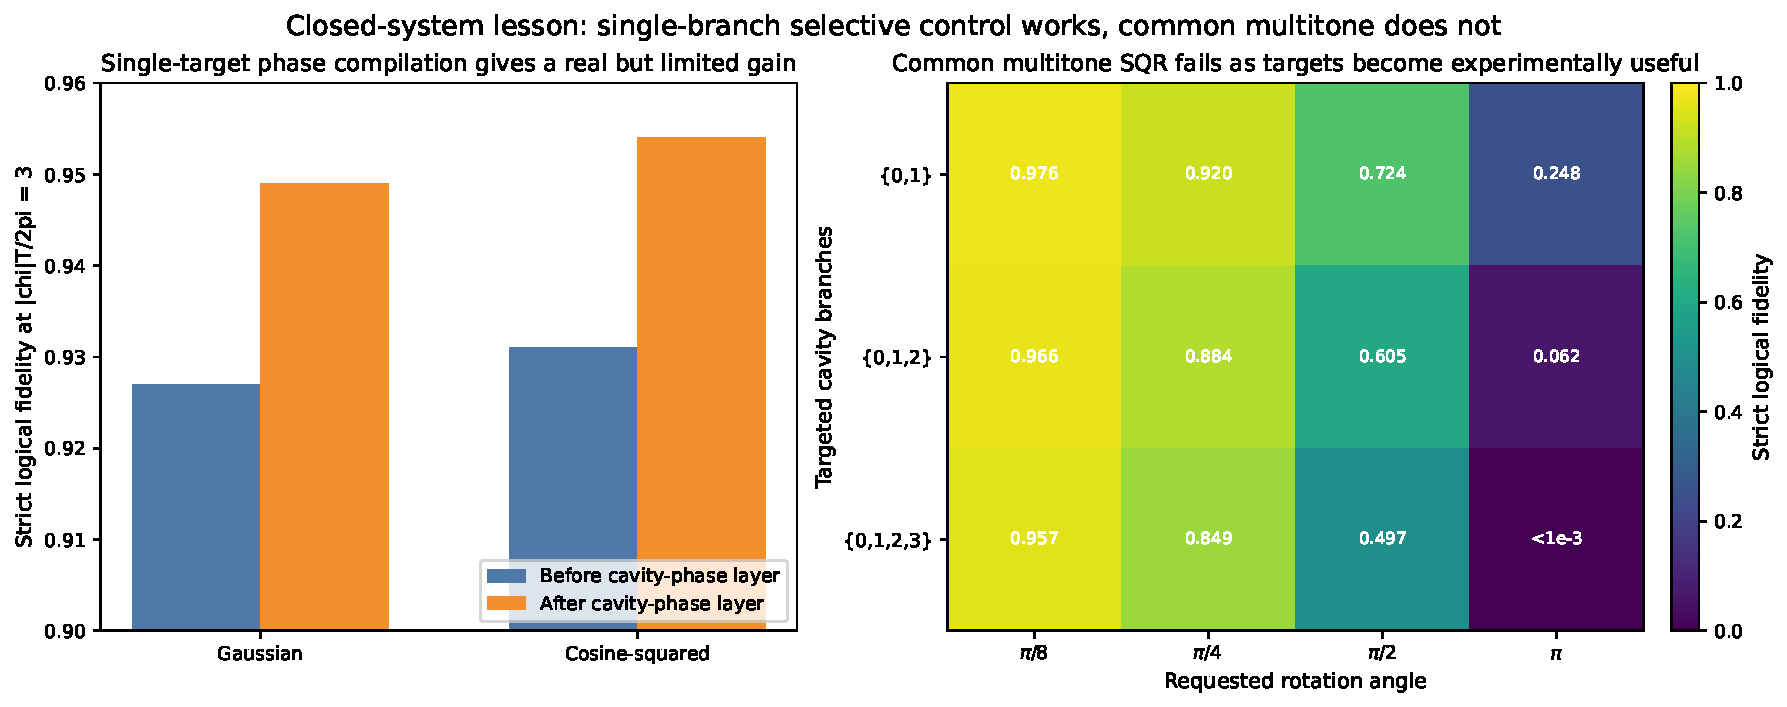
\includegraphics[width=\textwidth]{sqr_control_summary.pdf}
\caption{Closed-system summary for experiment design. Left: a cavity-only phase layer improves strict logical fidelity for single-target SQR on enlarged logical windows, but only by a few points. Right: common multitone simultaneous SQR rapidly loses usefulness as the requested angle and number of addressed branches increase. The natural practical conclusion is to keep SQR as a single-branch primitive and sequence it, rather than attempting common-waveform multi-branch control.}
\label{fig:sqr_control_summary}
\end{figure}

% ══════════════════════════════════════════════════════════
% 6. RESULTS: OPEN-SYSTEM PERFORMANCE
% ══════════════════════════════════════════════════════════
\section{Open-System SQR Under Realistic Noise}

\subsection{Realistic Multilevel Replay}

Under the explicit multilevel model $(T_{1,ge}, T_{1,fe})=(\SI{30}{}, \SI{10}{})\,\mu$s, the square-family SQR becomes the best practical replayed family: mean target fidelity averaged over $1\le |\chi|T/2\pi\le 5$ is $0.898$, compared with $0.891$ for cosine-squared and $0.877$ for Gaussian. The ranking change from the closed system occurs because shorter square pulses suffer less from decoherence despite their broader spectral width.

With storage thermal occupation $n_\mathrm{th,s}=0.02$, the best operating point is a short square-family gate near $|\chi|T/2\pi=1$ with mean target fidelity $\mathbf{0.944}$.

The thermal sweep shows gradual degradation: mean target fidelity at $|\chi|T/2\pi=2$ decreases from $0.924$ ($n_\mathrm{th}=0$) to $0.921$ ($n_\mathrm{th}=0.02$) to $0.909$ ($n_\mathrm{th}=0.10$).

\subsection{Purcell Budget}

The readout-chain analysis shows the Purcell filter is essential. Without the filter, the Purcell-limited $T_1$ spans $1.66$--$\SI{166}{\micro s}$ over the detuning sweep, potentially dominating the intrinsic transmon lifetime. With the filter, the Purcell-limited $T_1$ spans $2.9\times 10^5$--$2.9\times 10^9\,\mu$s, keeping the measurement chain contribution negligible.

\subsection{GRAPE Under Noise}

Archived closed-system GRAPE controls replayed through the stabilized noisy simulator path retain a clear advantage over parametric baselines:

\begin{table}[H]
\centering
\caption{GRAPE noisy target fidelities vs.\ best parametric (square) baseline.}
\begin{tabular}{@{} l c c c c @{}}
\toprule
$|\chi|T/2\pi$ & 1 & 2 & 3 & 5 \\
\midrule
GRAPE (noisy replay) & 0.978 & 0.958 & 0.941 & 0.907 \\
Square (noisy replay) & 0.944 & 0.924 & 0.898 & 0.850 \\
\bottomrule
\end{tabular}
\label{tab:grape_vs_parametric}
\end{table}

GRAPE outperforms the best parametric baseline by $\Delta F \approx 0.03$--$0.06$ across the sampled window, confirming it as a useful practical upper bound. This advantage comes from the GRAPE optimizer's ability to find controls that remain robust when replayed through noise, not from direct noisy-objective optimization (which is not yet supported).

\subsection{Three-Mode Concurrent Readout}

Concurrent readout degrades the reduced logical fidelity significantly, even with the conservative $\chi_{sr}=0$ assumption:

\begin{table}[H]
\centering
\caption{Reduced logical fidelity under concurrent readout (square family, $|\chi|T/2\pi=3$).}
\begin{tabular}{@{} l c c c @{}}
\toprule
Readout amplitude $\varepsilon_r/2\pi$ (MHz) & 0.5 & 1.0 & 2.5 \\
\midrule
Reduced fidelity & 0.822 & 0.726 & 0.632 \\
Storage coherence ratio & 0.961 & 0.961 & 0.961 \\
\bottomrule
\end{tabular}
\label{tab:concurrent_readout}
\end{table}

The storage coherence metric remains near unity, indicating the penalty comes from spectator degradation mediated by the full transmon--storage--readout dynamics, not direct storage dephasing.

Figure~\ref{fig:sqr_noise_summary} summarizes the noisy-control decision surface. The best parametric family is the short square pulse, GRAPE remains a useful upper bound, and concurrent readout extracts a clear fidelity tax even before a physical storage--readout cross-Kerr is added.

\begin{figure}[H]
\centering
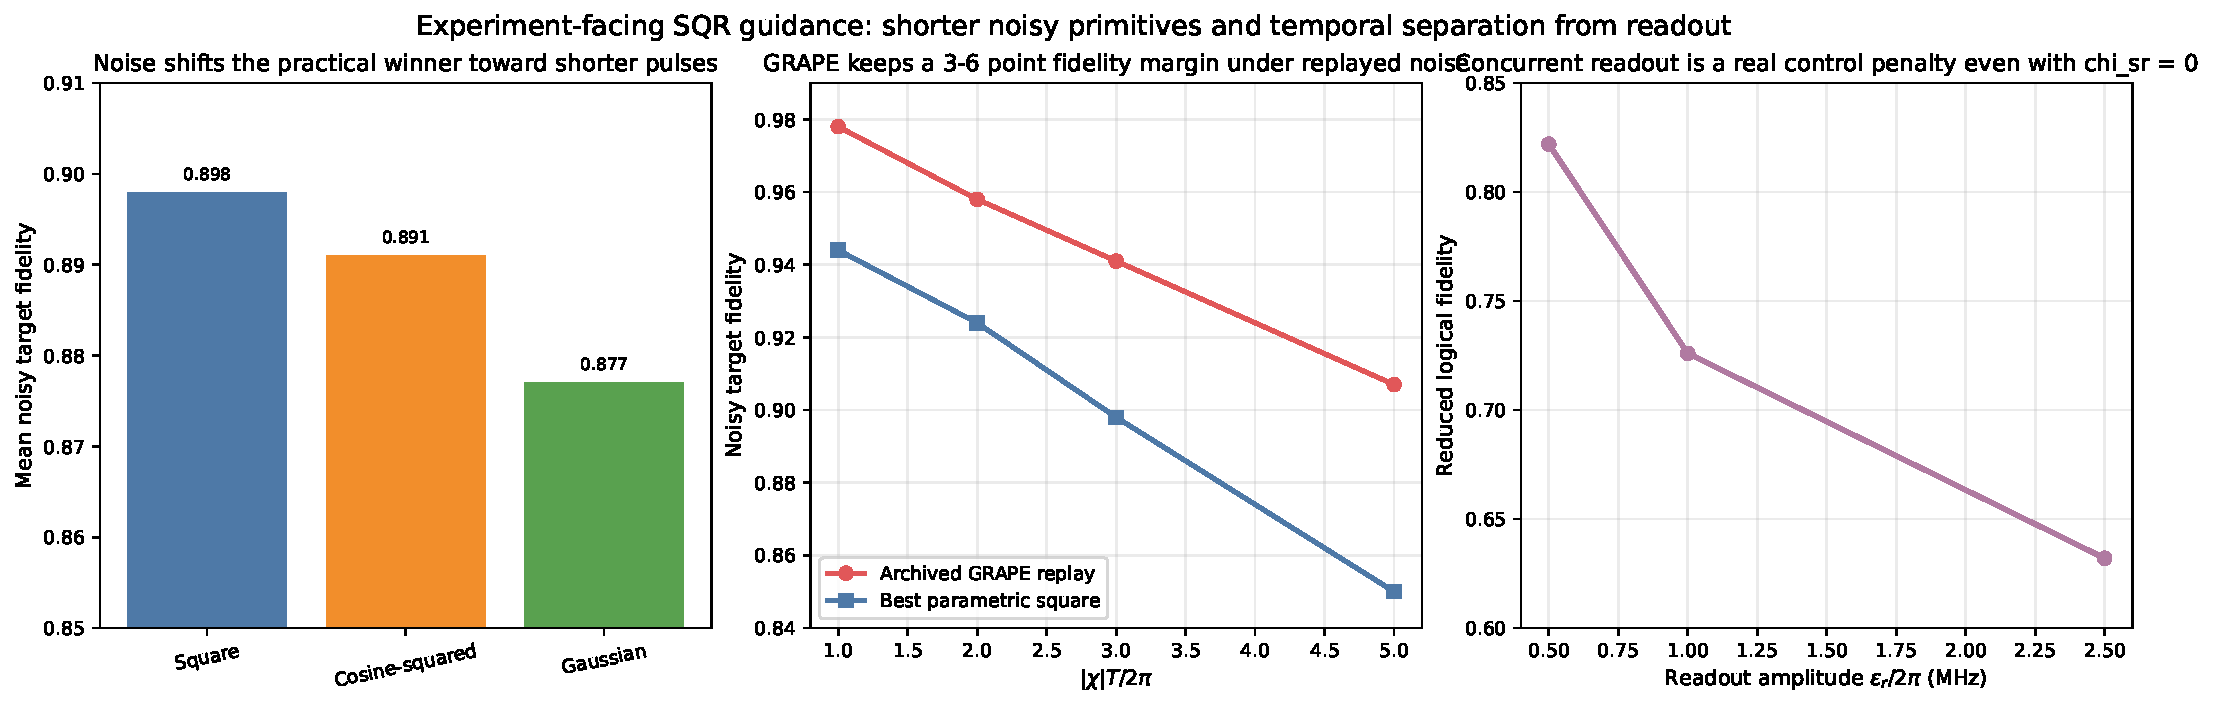
\includegraphics[width=\textwidth]{sqr_noise_summary.pdf}
\caption{Noise-aware SQR design summary. Left: family-average noisy ranking favors the shortest square-family primitive. Middle: archived GRAPE controls keep a clear noisy-replay advantage over the best parametric square baseline. Right: concurrent readout substantially degrades the reduced logical fidelity, supporting temporal separation of readout and selective gates whenever the experiment allows it.}
\label{fig:sqr_noise_summary}
\end{figure}

% ══════════════════════════════════════════════════════════
% 7. VALIDATION
% ══════════════════════════════════════════════════════════
\section{Validation}

\subsection{Sanity Checks}
Leakage across the full closed-system baseline scan stays below $7.4\times 10^{-5}$. GRAPE achieves $F\approx 1$ for cphase-SQR at all durations, confirming the system is controllable. The simultaneous multitone study independently verifies negligible leakage ($\max|f\rangle$ population $7.08\times 10^{-9}$) and perfect block preservation ($0.999998$), isolating the failure to the rotation mechanism. Monotonic loss trends are observed in the open-system replay.

\subsection{Convergence Analysis}
Closed-system results are stable across solver time-step refinement and cavity truncation increases ($n_\mathrm{cav}=6\to 10$). The simultaneous multitone study verified convergence in both $dt$ and $n_\mathrm{cav}$ and included qutrit spot-checks. GRAPE validation used representative reruns confirming consistency between archived and fresh controls. The open-system study verified that legacy single-$T_1$ and explicit multilevel models agree qualitatively, with the multilevel model providing sharper identification of the practical operating window.

\subsection{Literature Consistency}
The closed-system SQR results are consistent with the SNAP and selective-gate literature~\cite{heeres2015snap,krastanov2015universal,heeres2017logical}. The Purcell filter analysis agrees with standard textbook expectations~\cite{blais2021circuit}. The ranking change from cosine-squared to square under noise is physically reasonable: shorter selective pulses suffer less decoherence despite their broader spectral width.

% ══════════════════════════════════════════════════════════
% 8. DISCUSSION
% ══════════════════════════════════════════════════════════
\section{Discussion}

The unified SQR study delivers a clear hierarchy of practical insights. In the closed system, the conditional-phase SQR target with a cosine-squared envelope is the natural experimental primitive, approaching unit fidelity in the practical $|\chi|T/2\pi\sim 2$--$3$ regime. Phase compilation adds a useful but limited improvement for single-target operations on larger logical windows, while being entirely inappropriate for structured multi-branch short-gate problems.

The simultaneous multi-branch result is an important negative finding: common multitone waveforms cannot drive useful rotations on multiple branches simultaneously. This eliminates a potentially attractive control shortcut and redirects multi-branch SQR design toward sequential single-branch operations or fundamentally different waveform ansätze.

Under realistic noise, the practical recommendation shifts from cosine-squared to square-family SQR, with the optimal operating point moving to shorter durations ($|\chi|T/2\pi\sim 1$). GRAPE retains a meaningful advantage ($\Delta F\sim 0.03$--$0.06$) even when only replayed (not optimized) under noise, motivating future work on noise-aware GRAPE objectives. The concurrent readout penalty is substantial and argues for temporal separation of readout and SQR operations when possible.

For experiments pursuing broader transmon+cavity control, the report suggests a division of labor. Use cosine-squared cphase-SQR as the clean calibration primitive and benchmarking reference when coherence is not yet the bottleneck. Use short square-family SQR when ancilla lifetime and schedule pressure dominate. Do not treat common multitone simultaneous SQR as the route to scalable universal control. And if the experiment can tolerate the calibration complexity, treat GRAPE as the performance ceiling against which all parametric selective pulses should be judged.

% ══════════════════════════════════════════════════════════
% 9. CONCLUSION
% ══════════════════════════════════════════════════════════
\section{Conclusion}

\begin{table}[H]
\centering
\caption{Experiment-facing SQR primitive recommendations.}
\small
\begin{tabular}{@{} l l l l @{}}
\toprule
Regime & Recommended primitive & Fidelity & Notes \\
\midrule
Closed, $|\chi|T/2\pi\ge 2$ & Cosine-squared cphase-SQR & $>0.998$ & Best for benchmarking \\
Realistic noise & Square SQR, $|\chi|T/2\pi\sim 1$ & $0.944$ & Best parametric under noise \\
Enlarged logical window & Cosine-squared + cavity phase & $0.954$ (N=8) & Systematic $\Delta F\approx 0.02$ \\
Multi-branch simultaneous & \emph{Not viable} (common multitone) & --- & Sequential single-branch instead \\
Highest fidelity & GRAPE (closed, replayed noisy) & $0.978$ & Upper bound; not yet calibrated \\
\bottomrule
\end{tabular}
\normalsize
\end{table}

The main practical decision is therefore straightforward: calibrate SQR as a short, single-branch primitive and compose it with later phase cleanup, instead of chasing a one-shot multi-branch waveform. That route is shorter, more robust to ancilla decay, and better aligned with the experimentally relevant cphase-relaxed metric.

% ══════════════════════════════════════════════════════════
% 10. LIMITATIONS & FUTURE WORK
% ══════════════════════════════════════════════════════════
\section{Limitations and Future Work}

\subsection{Known Limitations}
\begin{itemize}
\item \textbf{GRAPE not optimized under noise.} Archived closed-system GRAPE controls are replayed through the noisy simulator but not re-optimized. Directly optimizing under a Lindblad objective could close the remaining $\sim$3--6\% gap. This requires new \texttt{cqed\_sim} functionality for noisy GRAPE objectives.
\item \textbf{Conservative three-mode assumptions.} The concurrent readout study uses $\chi_{sr}=0$, which underestimates the real penalty. Physical storage-readout cross-Kerr would worsen the concurrent readout degradation.
\item \textbf{Two-level transmon in closed system.} The closed-system and simultaneous multitone studies used $n_\mathrm{tr}=2$, limiting leakage assessment. The open-system study used $n_\mathrm{tr}=3$ and confirmed small but non-negligible $|f\rangle$ effects.
\item \textbf{Single device parameter set.} All results use one $\chi/\alpha$ ratio. The optimal envelope family may differ for devices with significantly different dispersive coupling.
\end{itemize}

\subsection{Suggested Improvements}
\begin{itemize}
\item \textbf{[P1 $|$ HIGH]} Implement noise-aware GRAPE optimization in \texttt{cqed\_sim} and compare directly against parametric baselines under identical noise assumptions.
\item \textbf{[P1 $|$ MEDIUM]} Repeat the three-mode study with physical $\chi_{sr}\ne 0$ to get realistic concurrent readout penalties.
\item \textbf{[P2 $|$ MEDIUM]} Design echoed/composite SQR sequences to reduce spectator branch-local qubit-$Z$ structure without sacrificing cavity-phase properties.
\item \textbf{[P2 $|$ MEDIUM]} Test SQR families in cat-code or binomial-code logical subspaces where the Fock-selective advantage may change.
\item \textbf{[P2 $|$ LOW]} Extend the enlarged-window phase compilation study to $N=12$+ to assess scalability.
\item \textbf{[P3 $|$ HIGH]} Build a calibrated GRAPE pulse-export pipeline for hardware replay.
\end{itemize}

\subsection{Open Questions}
\begin{itemize}
\item Can the corrected-parameterization multitone $(d_\lambda, d_\alpha, \delta\omega)$ close the gap to GRAPE in the all-branch case, or does the structured-ansatz ceiling persist independent of parameterization?
\item Why does square-family outperform cosine-squared under realistic noise despite being suboptimal in the closed system at longer durations? Is the effect purely decoherence-driven, or does spectral weight distribution matter?
\item At what logical window size does the linear cavity-phase profile break down?
\end{itemize}

% ══════════════════════════════════════════════════════════
% REFERENCES
% ══════════════════════════════════════════════════════════
\bibliographystyle{unsrtnat}
\bibliography{references}

\end{document}
